%
%%%%%%%%%%%%%%%%%%%%%%%%%%%%%%%%%%%%%%%%%%%%%%%%%%%%%%%%%%%%%%%%%%%%%%%%%%%%%%%
% Fractio of gluon splitting in data
%%%%%%%%%%%%%%%%%%%%%%%%%%%%%%%%%%%%%%%%%%%%%%%%%%%%%%%%%%%%%%%%%%%%%%%%%%%%%%%
%
\chapter{Fraction of double $b$-hadron jets in data}\label{ch:gbbfraction}

%------------------------------------------------------------------------
\section{Unbinned maximum likelihood fits}\label{sec:LLFits}
%------------------------------------------------------------------------


We measure in our experiments a number of observables $x_i$ and we want to determine one or more parameters $p_i$ from the data, such as the number of signal and background events, for instance. We describe the distribution of our observables by a probability density function (PDF), which is a function of both the observables and the parameters, $F(\vec{x},\vec{p})$. We choose the PDF based on some guess about what function would match the data.
We vary the parameters to make the PDF match the actual distribution of the observables as well as possible. This is called a ``fitting''.


We are familiar with the least-squares fit:
%
\begin{itemize}
\item
Bin data into a histogram, minimize $\chi^2 = \sum_i (y_i - y_{expected})^2 / \sigma^2_i$
\item
For a histogram, $y_i = N_i$, and $\sigma_i=\sqrt{N_i}$ (Poisson statistics in each bin)
\end{itemize}
%
We will use a different technique for fitting, an ``unbinned maximum likelihood fit''.  A least-squares fit mimics a maximum-likelihood fit if the bins are narrow and all bins have many events.  

Weights are supported in unbinned datasets. %But use with care. Error analysis in ML fits to weighted unbinned data can be complicated...


%Binned or unbinned MF fit. %Roofit presentation page 112
%In most RooFit applications it doesn't matter. Internally binned data is represented the same way as unbinned data, a ROOT TTree with the bin coordinates.

Maximum likelihood (ML) information only parametrizes the shape of a 
distribution (i.e. one can determine fraction of signal events from 
MC fits but no number of signal events).

%\subsubsection{Extended maximum likelihood fits}

The extended version of the maximum likelihood approach adds an extra term
allowing the estimation of %the absolute number of signal/background events.
a parameter that represents the number of events in the sample, $N_{exp}$.
The extra term describes the probability of observing the actual number of events, $N_{obs}$, given this parameter. This probability is described by the Poisson distribution
%
\begin{equation}
P(N_{obs},N_{exp}) = \frac{1}{N!} \cdot N_{exp}^{N_{obs}} \cdot exp(-N_{exp}),
\end{equation}
%
and we refer to the likelihood including this factor as the ``extended likelihood''
%
\begin{equation}
\tilde{\mathcal{L}}(\vec{x},N_{obs};\vec{p},N_{exp}) \equiv P(N_{obs},N_{exp}) \cdot \mathcal{L}(\vec{x};\vec{p})
\end{equation}
%

The aim of the maximum-likelihood method is to find the number of signal and background events in a given data sample that maximises the likelihood function, $\mathcal{L}$:
%
\begin{equation}
\mathcal{L} =  \frac{e^{-\sum n_j}}{N!} \prod^N_{i=1}\sum^m_{j=1} n_j  \mathcal{P}_j
\end{equation}
%
where $\mathcal{P}_j$ is the total probability for each of the $m$ hypothesis, $n_j$ is the number of events for the $j^{th}$ hypothesis, and $N$ is the total number of input data points. Note that the above expression represents the extended likelihood function, since it contains the relevant Poisson term.  The probabilities $\mathcal{P}_j$ are just the total PDFs that represent the probability of observing an event of type $j$, based on a set of discriminating variables. 

Before doing any fitting, a set of cuts is imposed to the sample.  After the relevant PDFs have been found, they are use to form the likelihood function.  The fit then finds the values of $n_j$, the number of events for each hypothesis $j$.



%\subsubsection{Fitting and likelihood minimization}

Performing a fit consists of minimizing the negative log-likelihood of a PDF calculated over a data set
%
\begin{equation}
-\log \mathcal{L} (\vec{p}) = \sum_k F(\vec{x}_k;\vec{p})
\end{equation}
%
with respect to the model's parameters.  The RooFitTools package uses the MINUIT\cite{MINUIT} algorithms to find the minimum of this function and estimate the errors in each parameter.  %fitTo() method returns an interger status code which is non-zero if the fit fails to converge normally.
%In order to assess the goodness of a fit one can compare the minimum value of the negative log-likelihood function with the expected distribution of values for samples generated according to the fit model (using the Monte Carlo study methods).


To increse the chances of proper convergence, it is important to provide reasonable initial estimates for the parameters to be fitted.

%\subsubsection{Model}

Most realistic data description models are sum of multiple components, e.g. signal and background. Mathematically, the sum of two probability density functions is  also a normalized probability density function as  long as the coefficients add up to 1, % (or to the total number of events for an extended maximum likelihood fit),
%
\begin{equation}
M(x) = f_{sig} \cdot S(x) + (1-f_{sig}) \cdot B(x),
\end{equation}
%
or generically for N components:
%
\begin{equation}
S(x) = c_0 \cdot F_0(x) + c_1 \cdot F_1(x)+...+c_{n-1}F_{n-1}(x)+ (1-\sum^{n-1}_{i=1}c_i) F_n(x)
\end{equation}
%
If the sum of these coefficients becomes larger than one, the remainder coefficient will be assigned a negative fraction. As long as the summed p.d.f is greater than zero everywhere, this is not ill-defined. %but may pose some problems in the interpretation

For the extended fit, 
%
\begin{equation}
N_{sig} = f_{sig} \cdot N_{exp}
\end{equation}
%
\begin{equation}
N_{bkg} = (1-f_{sig}) \cdot N_{exp}
\end{equation}
%
so that the extended ML procedure estimates the number of singal and background events rather than a signal fraction and a total number of events.
%The uncertainties in the yields reported by the fit will include the statistical (      )                  N                    uncertainty.

Estimated Distance to Minimum
should be small O(10-6)
%------------------------------------------------------------------------
\section{Results}\label{sec:FitsResults}
%------------------------------------------------------------------------

The likelihood template fits are performed using an unbinned maximum likelihood technique.

The likelihood Monte Carlo templates were derived from the simulated dijet sample described in Section~\ref{sec:analysis}.

Templates of likelihood were constructed for $b$, $c$, $b\bar{b}$, $c\bar{c}$ and light MV1 tagged jets separately, and these were fit to the likelihood distribution in data to obtain the fraction of single $b$, merged $b$, single $c$, merged $c$ and light jets in the data sample.  The fit is done by adjusting the relative constributions of the different templates such that the sum of them best describes the likelihood shape in data. A separate fit was performed for each $\pt$-bin.  The templates were derived from all jets passing the selection criteria defined in Section~\ref{sec:EventSelection}.


Different combinations of templates were used to fit the likelihood distribution in data. 
The sensitivity of the fit to fixing the ratio of the $c$- to $b$-flavour fractions to the value extracted from the simulation was investigated by carrying out separate fits with 5 and 3 free parameters. This was motivated by the fact that templates for single $c$- (merged $c$-)  and single $b$-jets (merged $b$-jets) look very similar leading to inestabilities in the fitted $b$- and $c$-flavour fractions.
%PARA JUSTIFICAR QUE HACEMOS LOS FITS CON 3 PARAMETROS PODEMOS MOSTRAR LOS HISTOS Y DECIR QUE LAS CORRELACIONES SON MUY GRANDES (PONER NUMEROS). EN ALGUN MOMENTO TENDRA QUE HABER UN C-TAGGER.  EN DIJET TENEMOS SINGLE-C'S, EN TTbar NO HAY C'S, SI HAY MERGED-C PERO ES ALGO QUE QUEREMOS REMOVER DE TODAS MANERAS.




True fractions derived in {\sc Pythia} simulation as a functin of the jet $\pt$ is shown in Fig.~\ref{fig:truefractions}.


\begin{figure}[tp]
\centering
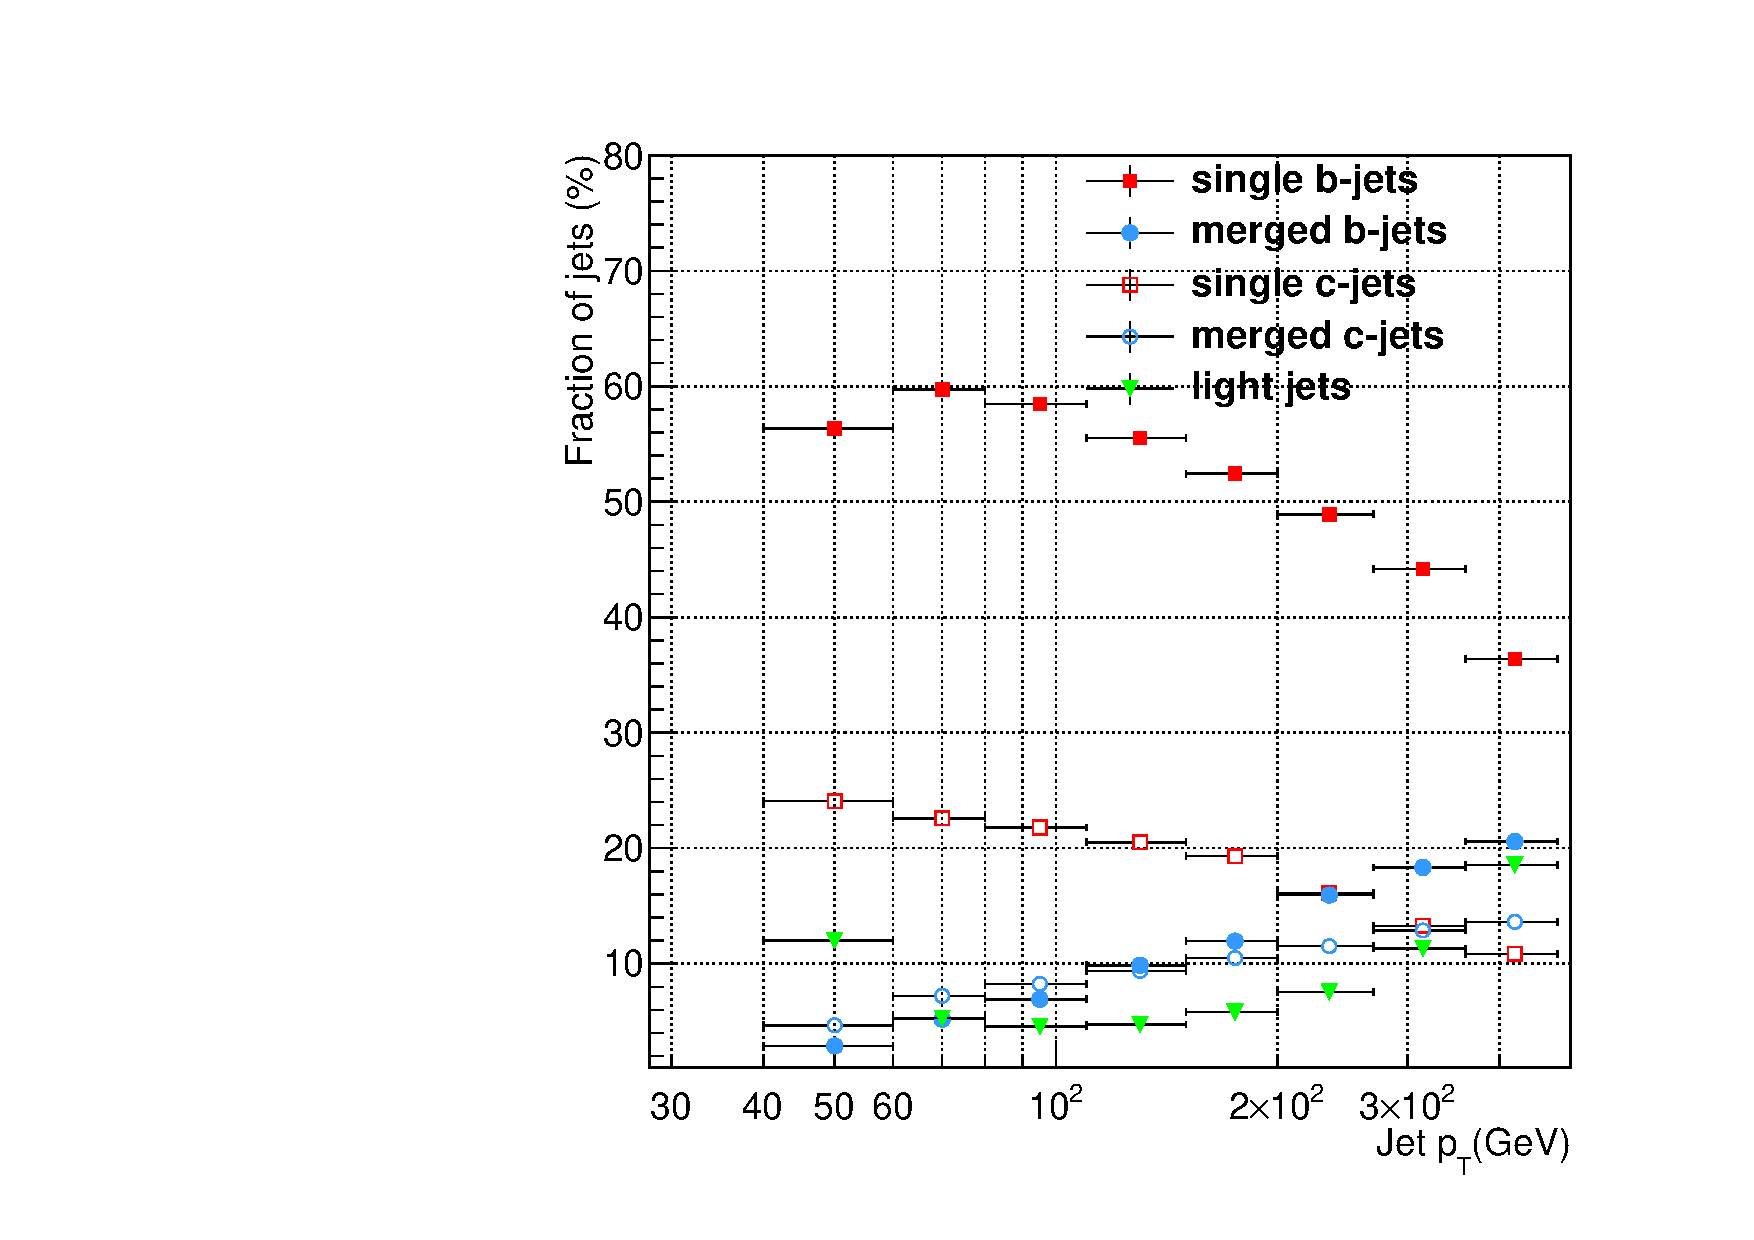
\includegraphics[width=0.7\textwidth]{TrueFractions_NominalPythia.pdf}
%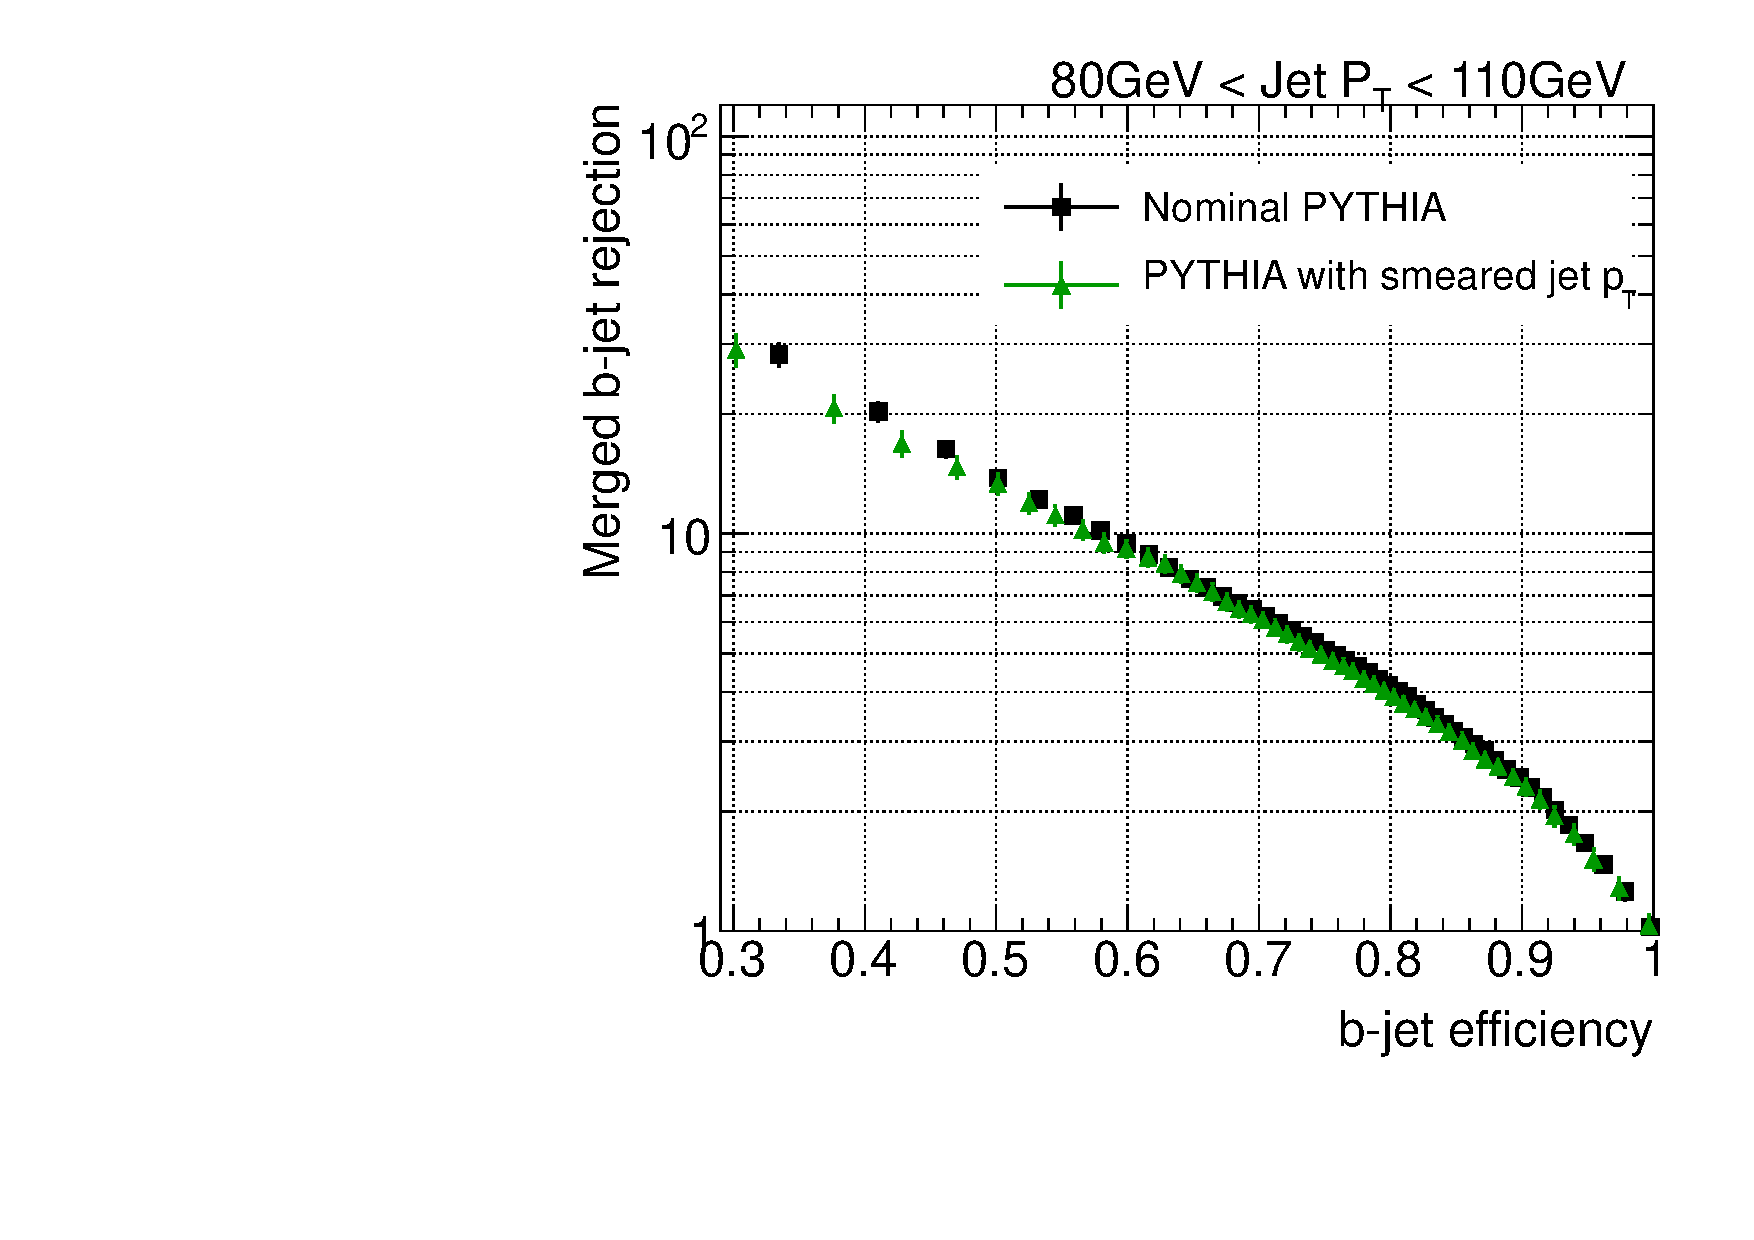
\includegraphics[width=0.49\textwidth]{FIGS/systematics/LlhoodKDE_ISO_SmearedJetPt_FIXEDBUGTest_rejvseff080.pdf}
\caption{Pythia predictions of the fractions of MV1 tagged $b$-, $b\bar{b}$-, $c$-, $c\bar{c}$, and light jets in a Monte Carlo dijet sample.}
\label{fig:truefractions}
\end{figure}




The results of the 3-parameter fits for all bins of $\pt$ are shown in table~\ref{tb:fitfractions}.

The fit results are shown in Figures~\ref{fig:fittemplates1} and~\ref{fig:fittemplates2}.


\begin{figure}[tp]
\centering
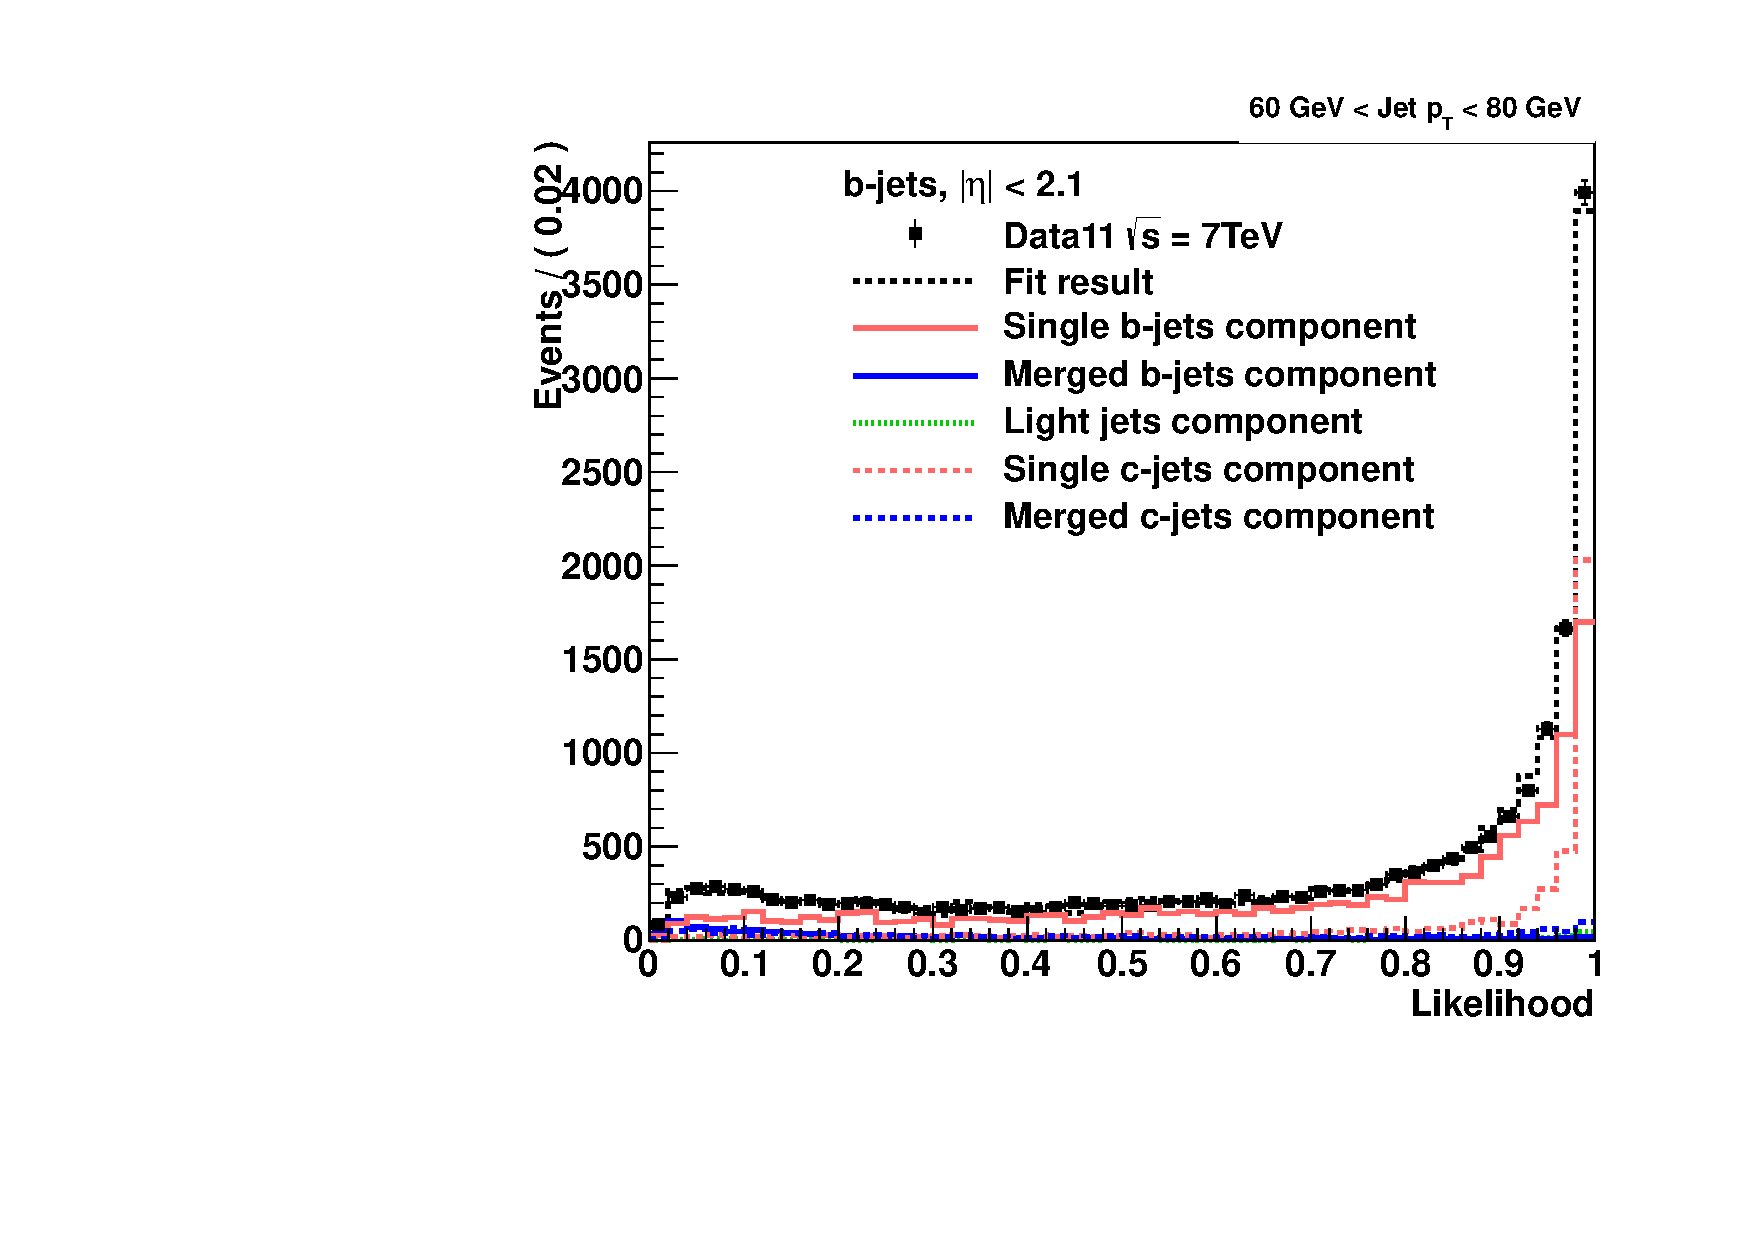
\includegraphics[width=0.7\textwidth]{FIGS/Fits/LikelihoodFit_3param_ETAFull_Bin1.pdf}
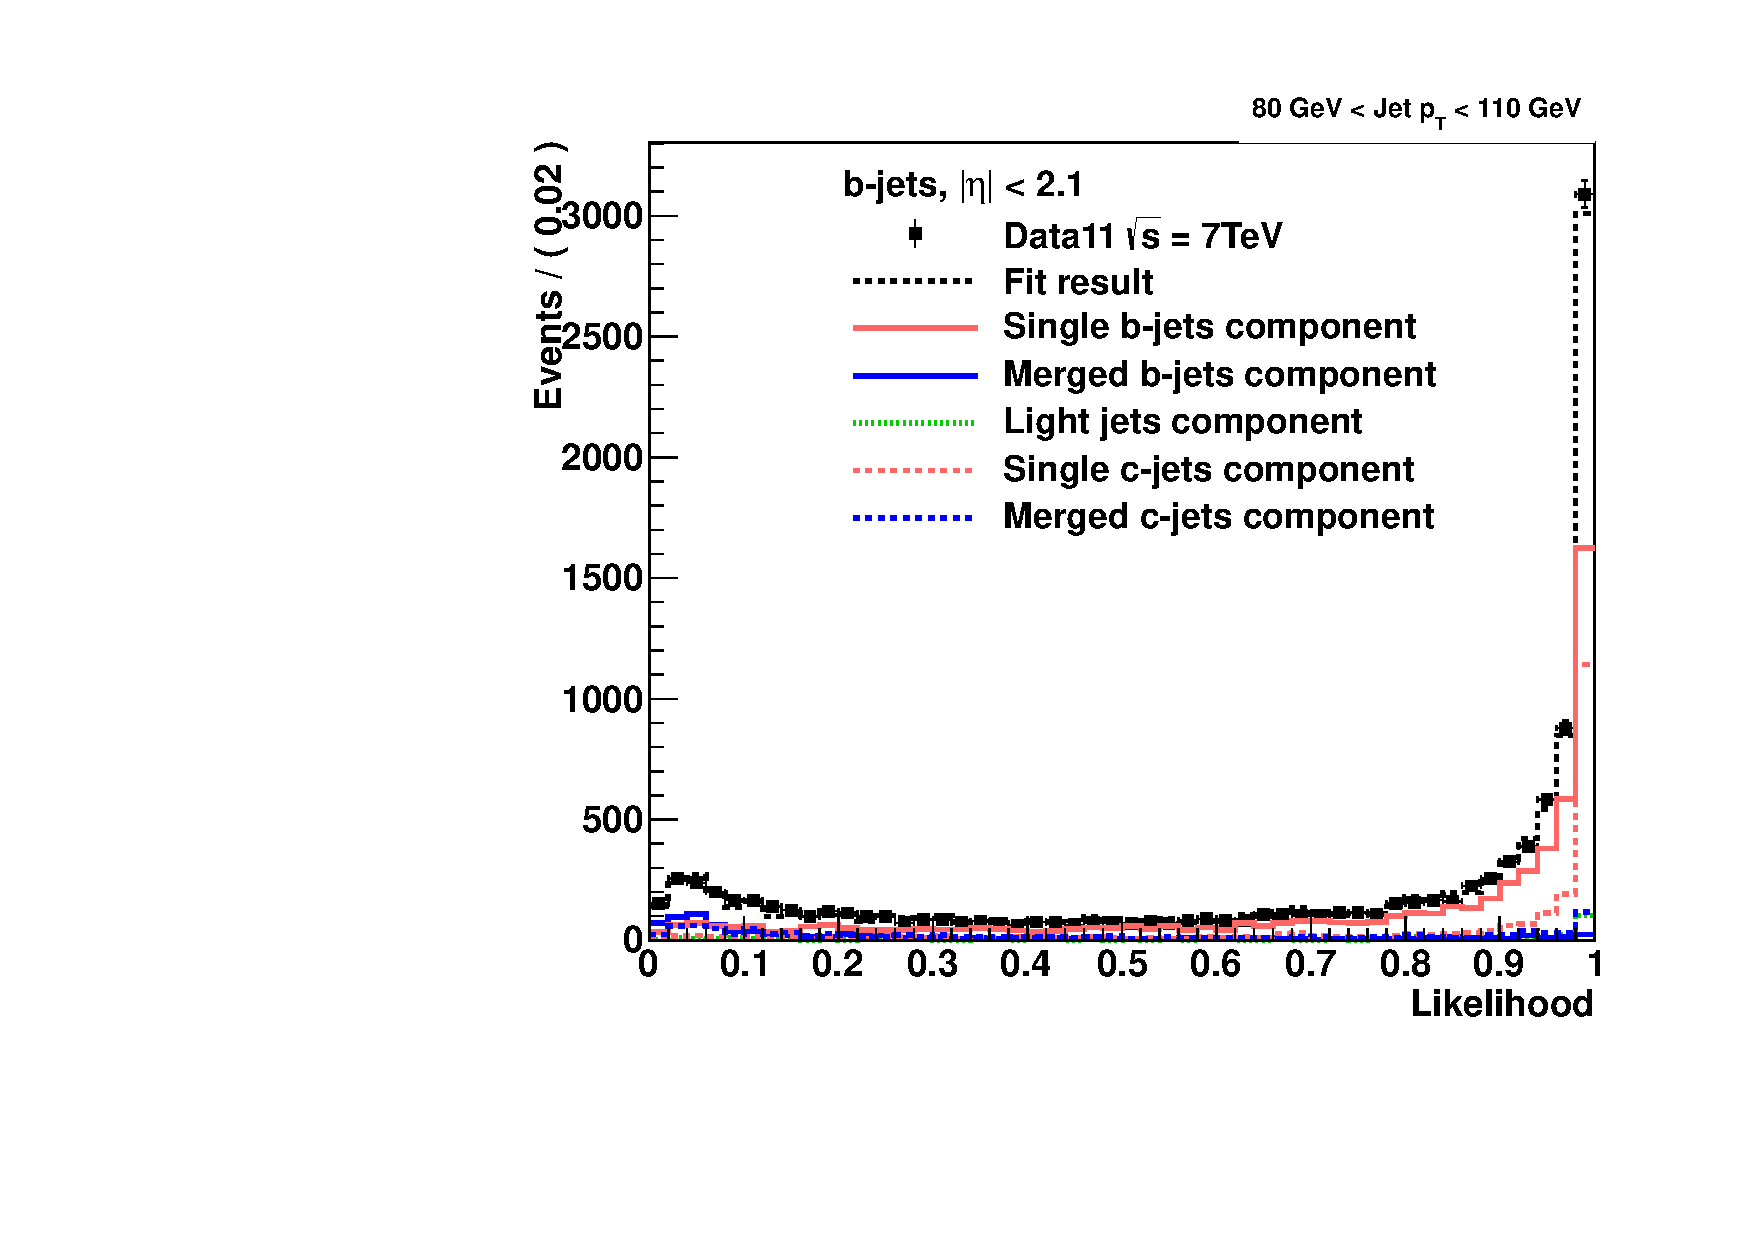
\includegraphics[width=0.7\textwidth]{FIGS/Fits/LikelihoodFit_3param_ETAFull_Bin2.pdf}
\caption{The results of template fits to the likelihood distribution in data. The fits shown here were performed on jets with $\pt$ between  60~GeV and 80~GeV, and 80~GeV and 110~GeV, using five templates of $b$-, $b\bar{b}$-, $c$-, $c\bar{c}$, and light jets.  The ratio of the $c$- to $b$-flavour fractions was fixed to the values observed in the simulation.  Uncertainties shown are for data statistics only.  }
\label{fig:fittemplates1}
\end{figure}



\begin{figure}[tp]
\centering
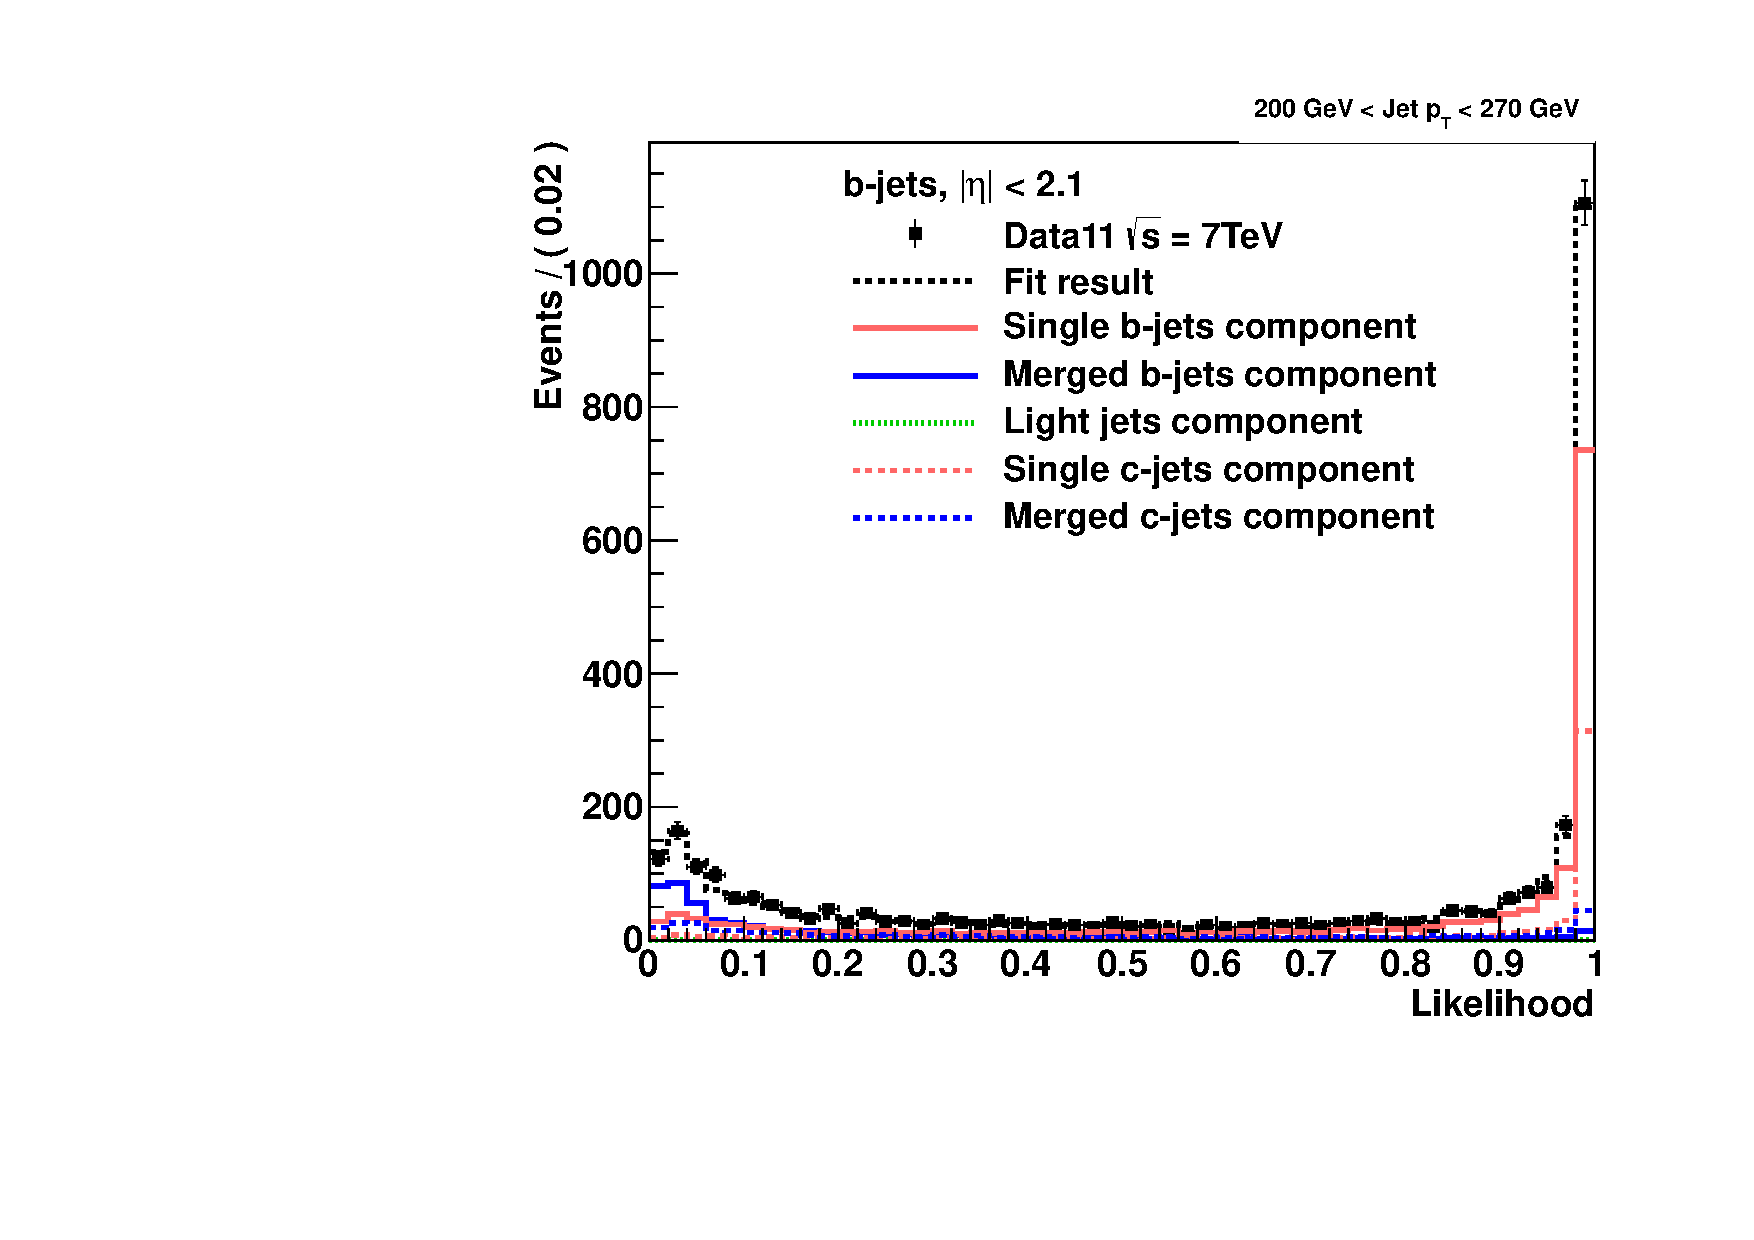
\includegraphics[width=0.7\textwidth]{FIGS/Fits/LikelihoodFit_3param_ETAFull_Bin5.pdf}
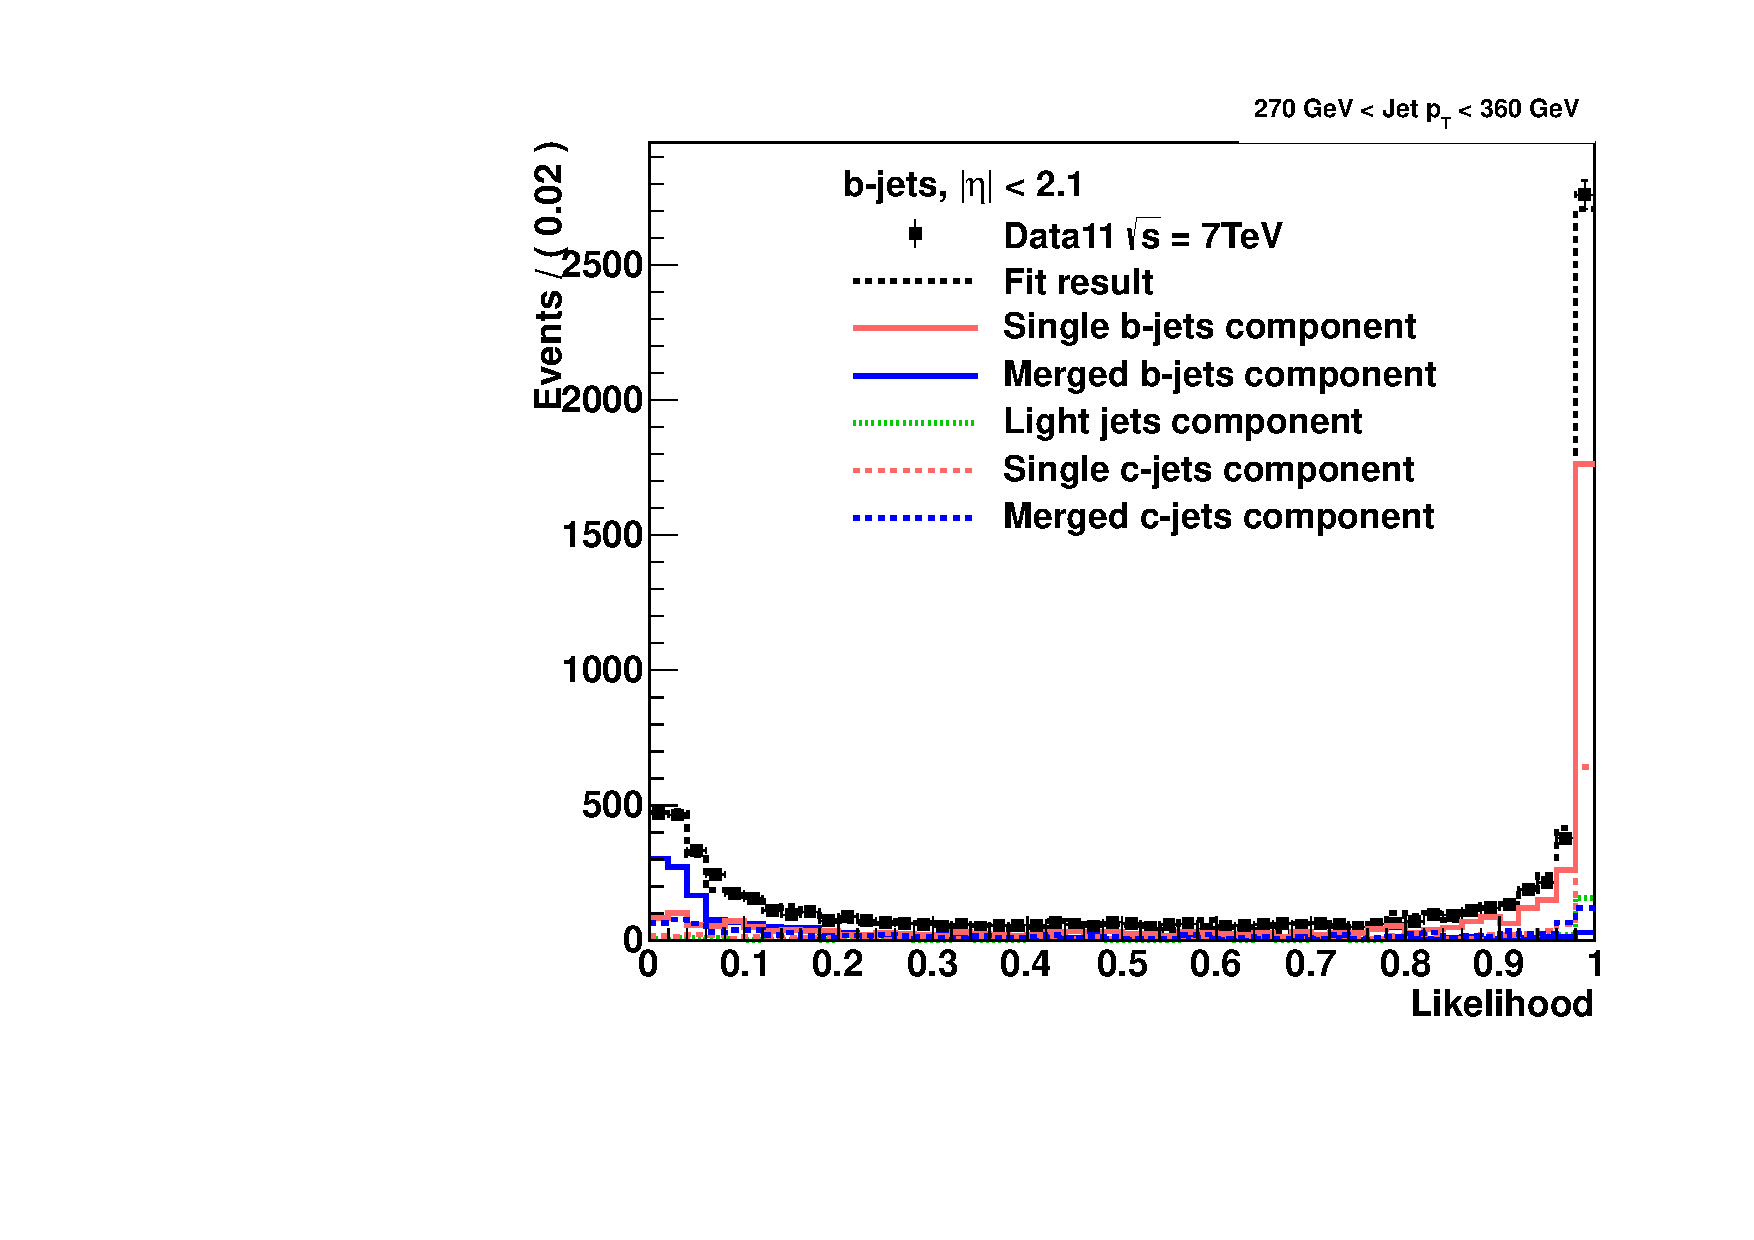
\includegraphics[width=0.7\textwidth]{FIGS/Fits/LikelihoodFit_3param_ETAFull_Bin6.pdf}
\caption{The results of template fits to the likelihood distribution in data. The fits shown here were performed on jets with $\pt$ between  200~GeV and 270~GeV, and 270~GeV and 360~GeV, using five templates of $b$-, $b\bar{b}$-, $c$-, $c\bar{c}$, and light jets.  The ratio of the $c$- to $b$-flavour fractions was fixed to the values observed in the simulation.  Uncertainties shown are for data statistics only.}
\label{fig:fittemplates2}
\end{figure}

\begin{table}[!hbt] %[h]
\renewcommand{\arraystretch}{1.2}
\centering
\begin{tabular}{ | c || c | c || c | c || c | c ||}
  \hline
  Jet $\pt$ & \multicolumn{2}{c||}{single $b$-jet} & \multicolumn{2}{c||}{merged $b$-jet} & \multicolumn{2}{c||}{~light jet~}\\ \cline{2-7}
    (GeV ) & fit result & ~stat.err. & fit result & ~stat.err. & fit result & ~stat.err.\\ \hline
   40 - 60 &  62\% &  3\%  &  ~~3\%  &  ~~1\% &  ~4\%  &  4\%   \\ 
   60 - 80 &  62\% &  1\%  &  5.2\%  &  0.4\% &  ~2\%  &  2\%   \\ 
   80 - 110&  57\% &  1\%  &  8.5\%  &  0.4\% &  ~3\%  &  2\%   \\ 
  110 - 150&  55\% &  2\%  &  ~13\%  &  ~~1\% &  ~1\%  &  4\%   \\ 
  150 - 200&  53\% &  3\%  &  ~15\%  &  ~~1\% &  ~0\%  &  4\%   \\ 
  200 - 270&  53\% &  5\%  &  ~17\%  &  ~~1\% &  -1\%  &  7\%   \\ 
  270 - 360&  48\% &  3\%  &  ~19\%  &  ~~1\% &  ~4\%  &  4\%   \\ 
  360 - 480&  39\% &  5\%  &  ~21\%  &  ~~1\% &  15\%  &  6\%   \\ \hline
\end{tabular}
\caption{Measured fractions of single, merged and light $b$-tagged jets in experimental data from 2011 run.}
\label{tb:fitfractions}
\end{table}







%------------------------------------------------------------------------
\section{Systematic uncertainties}\label{sec:FractionSystematics}
%------------------------------------------------------------------------




The systematic uncertainties affecting the method are mainly those that change the shape of the likelihood tamplates used to fit the sample composition. The following contributions were evaluated:

\begin{itemize}\addtolength{\itemsep}{-0.4\baselineskip}
\item
uncertainty in the track reconstruction efficiency;
\item
uncertainty in the jet transverse momentum resolution {\bf TO DO};
\item
uncertainty in the jet energy scale.
\item
heavy flavor fraction.
%the effect of jet isolation
%\item
%other $\Delta R$ cuts for B-labeling and matching
\end{itemize}


The systematic uncertainty originating from the jet energy scale is obtained by scaling the $\pt$ of each jet in the simulation up and down by one standard deviation, according to the uncertainty of the jet energy scale (see Section~\ref{sec:gbbSystematics}), and redoing the likelihood fits on data with the modified $b$, $c$, $b\bar{b}$, $c\bar{c}$ and light templates.


The systematic uncertainty originating from the jet  $\pt$ resolution is obtained by smearing the calorimeter jet $\pt$ in the simulation. The likelihood templates were rederived from this ``smeared'' sample, and the likelihood distribution in data was fit using these altered samples. The difference between the unsmeared and the smeared scenarios is taken as a systematic uncertainty. 

Changing the ratio of merged $c$ to merged $b$ fraction in 20\% only produced a marginal effect on the fit results. The total number of merged $c$ plus merged $b$ did not change showing that in reality we are measuring the fraction of merged $b+c$ together. The same result is expected if changing the single $c$/single $b$ ratio.


The systematic uncertainties are summarized in Table~\ref{tb:systematicsfits}. The largest ones arise from the jet energy scale and jet transverse momentum resolution. 
\begin{table}[!hbt] %[h]
\renewcommand{\arraystretch}{1.2}
\centering
\begin{tabular}{ | c | c |}
\hline
  ~~~~~~~Systematic source~~~~~~~ &~~Uncertainty~~\\ \hline
  track reconstruction efficiency  &    negligible\%        \\ 
  jet $\pt$ resolution  &    2\%        \\  
  jet energy scale  &    2\%        \\ \hline 
  flavour fractions  &    negligible        \\ \hline 
\end{tabular}
\caption{Systematic uncertainties.}
\label{tb:systematicsfits}
\end{table}





%------------------------------------------------------------------------
\section{Enriched samples in single and merged $b$-jets}\label{sec:Enriched}
%------------------------------------------------------------------------

\subsubsection{Enriched sample in merged $b$-jets}



\subsubsection{Enriched sample in single $b$-jets}

The results of performing the fits on an data sample enriched in single $b$-jets is shown in tables~\ref{tb:fitfractions2btagS} to ~\ref{tb:fitfractions2btagL}. The model fitted to the data agrees well within statistics %THE TEMPLATES WORK WELL!
and the result is in agreement with the predictions made by {\sc Pythia} on a sample with the same level o of enrichment.  % (PODRIAMOS DECIR QUE LA FRACCION DE FLAVOR CREATION ESTA BIEN SIMULADA POR PYTHIA)


The fit results are shown in Figures~\ref{fig:fitenriched2btag1} and Figures~\ref{fig:fitenriched2btag2}.


\begin{figure}[tp]
\centering
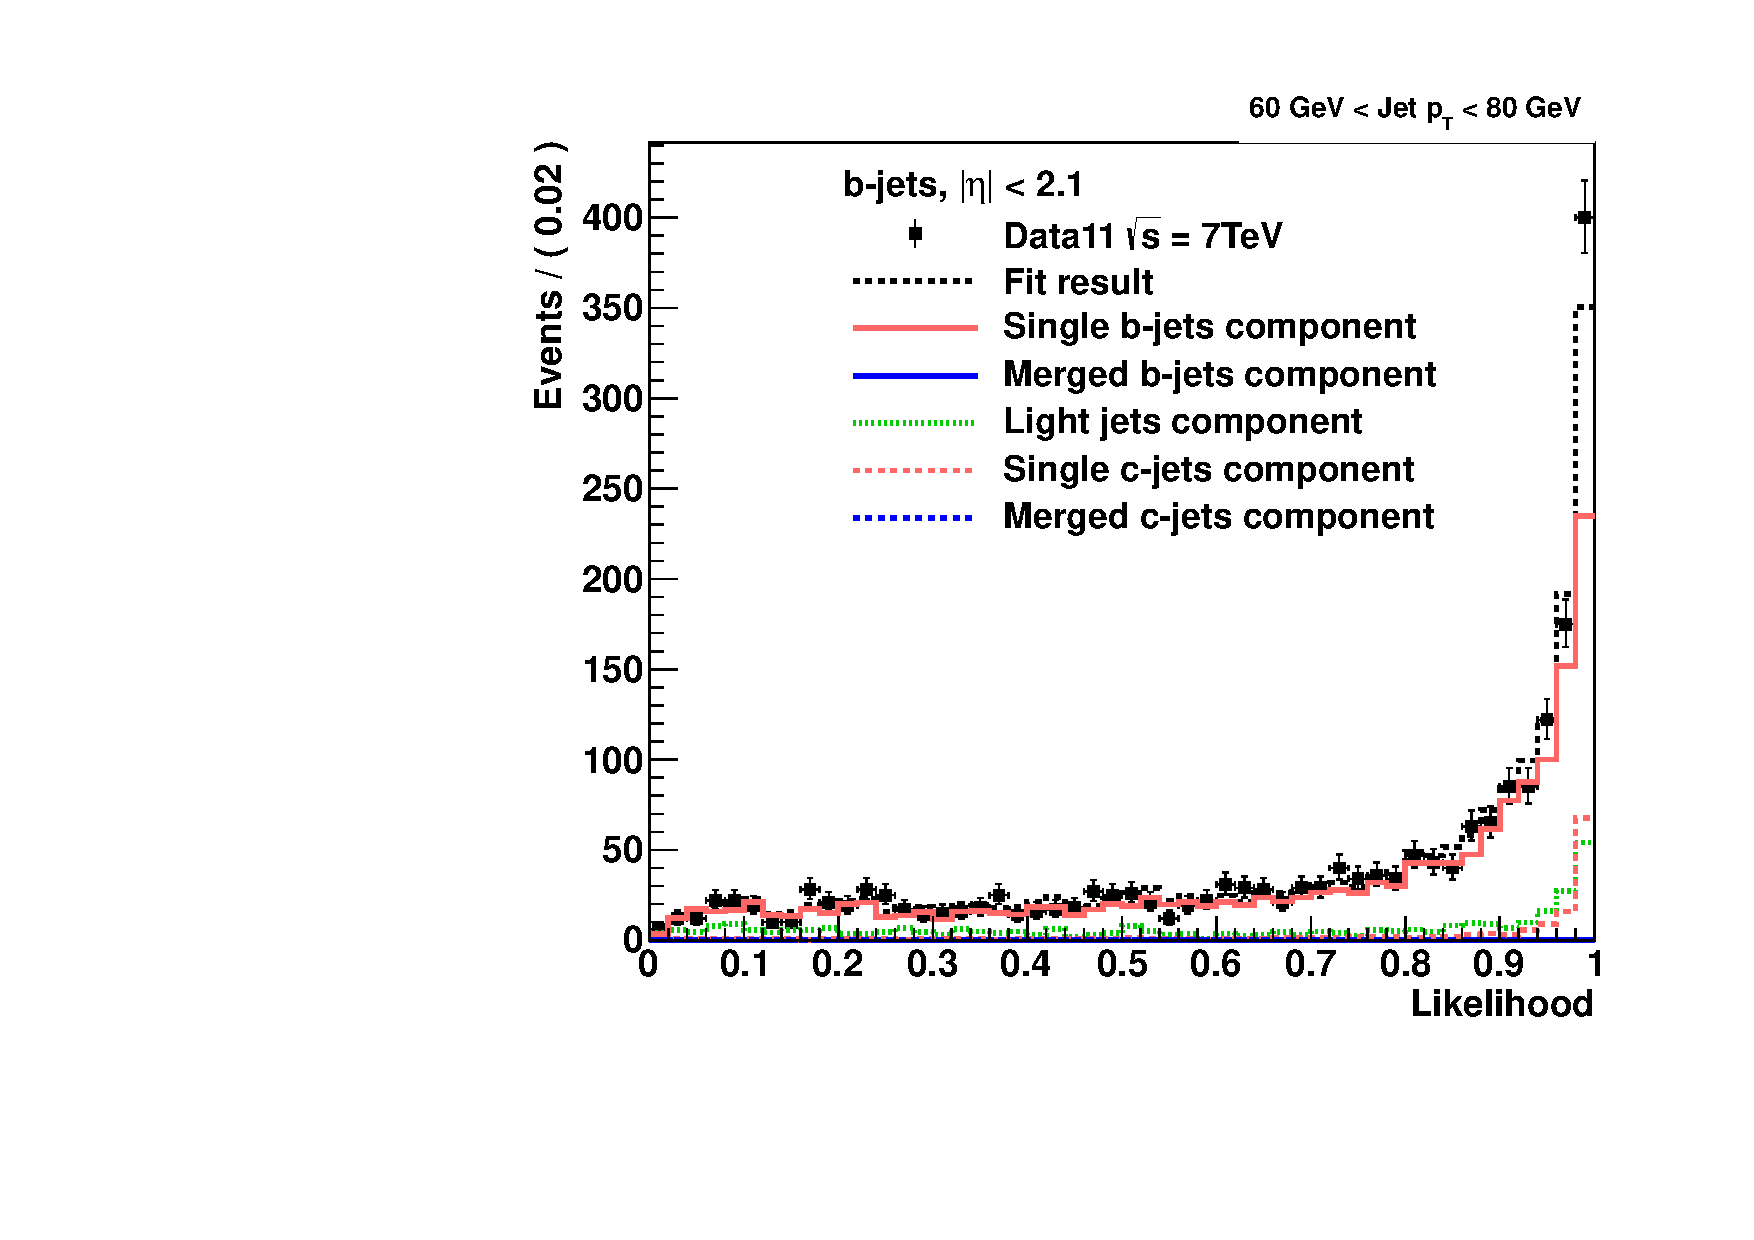
\includegraphics[width=0.7\textwidth]{FIGS/Fits/LikelihoodFit_3param_ETAFull_DataEnriched2btag_Bin1.pdf}
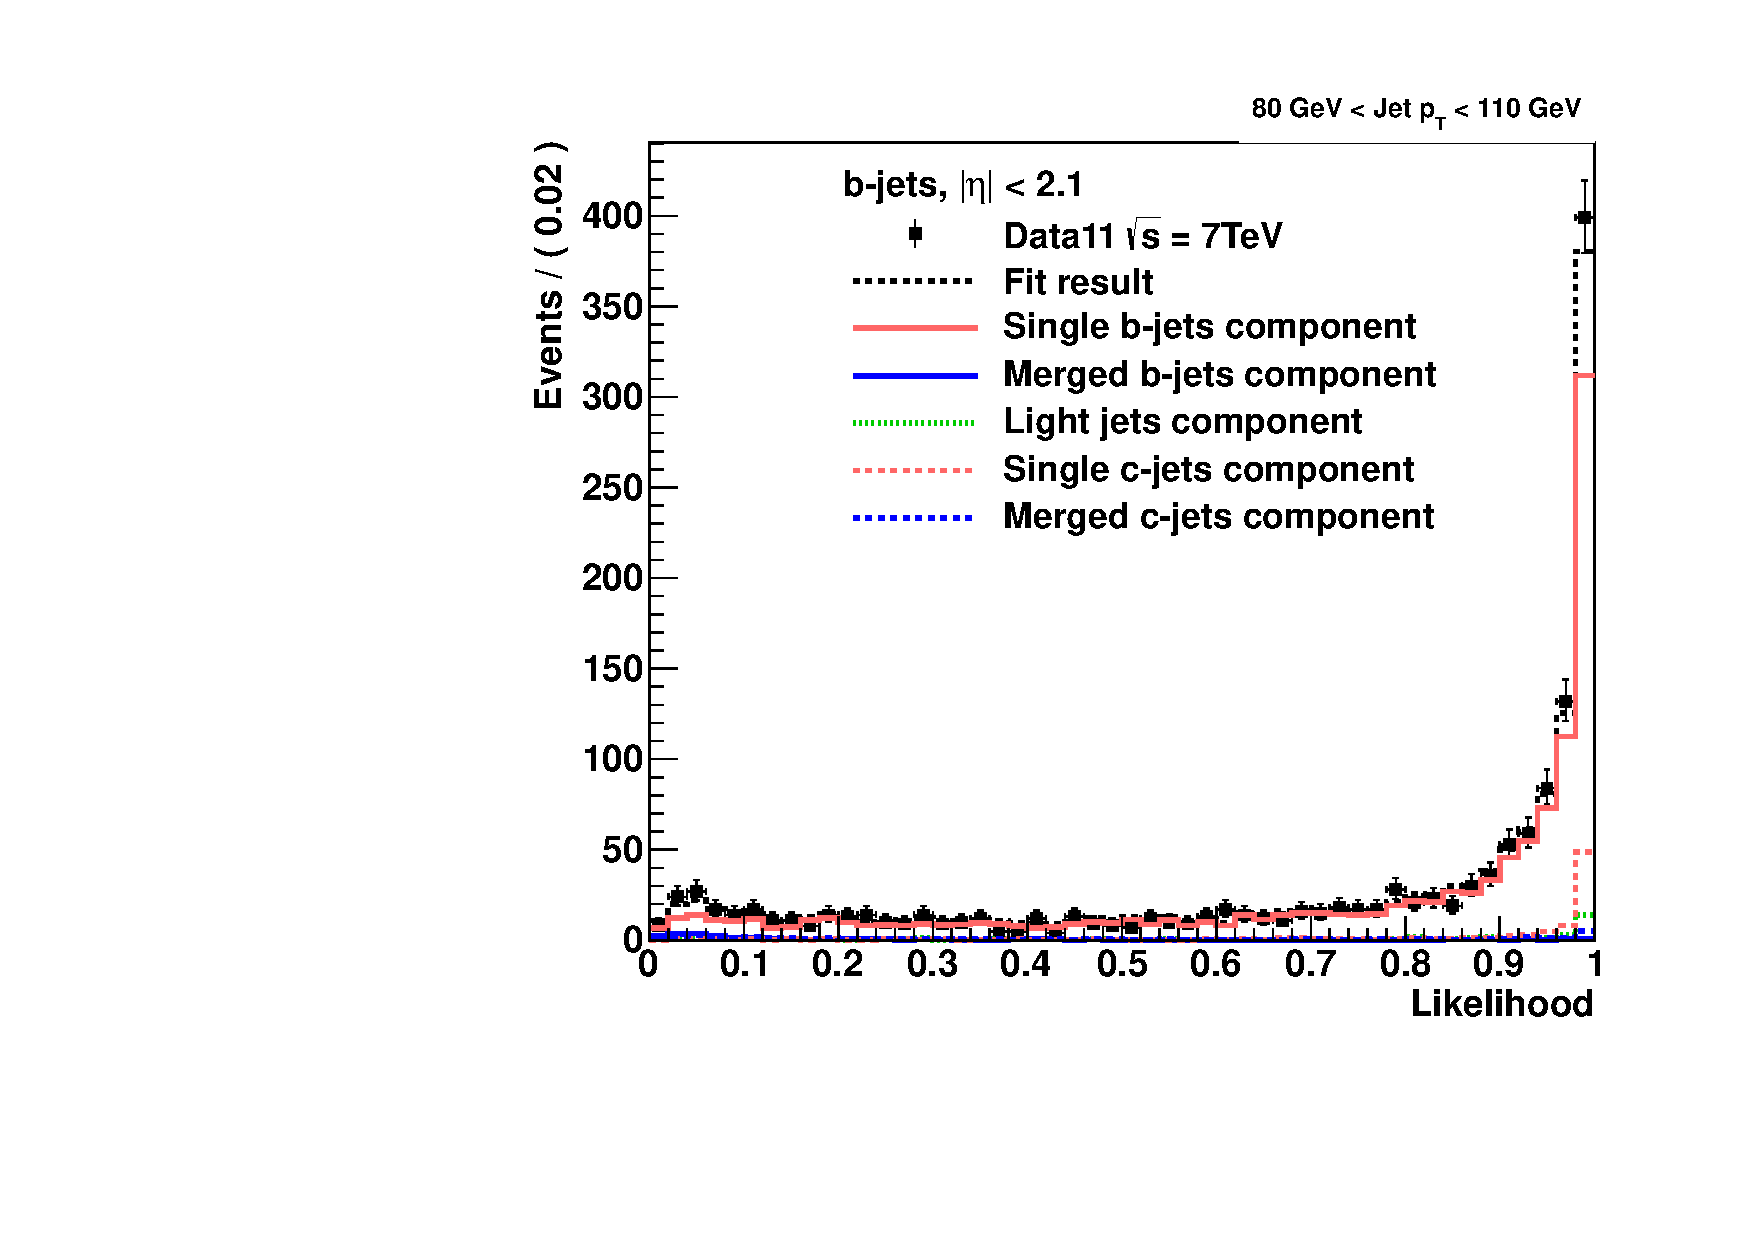
\includegraphics[width=0.7\textwidth]{FIGS/Fits/LikelihoodFit_3param_ETAFull_DataEnriched2btag_Bin2.pdf}
\caption{The results of template fits to the likelihood distribution in data enriched in single $b$-jets. The fits shown here were performed on jets with $\pt$ between  60~GeV and 80~GeV, and 80~GeV and 110~GeV, using five templates of $b$-, $b\bar{b}$-, $c$-, $c\bar{c}$, and light jets.  The ratio of the $c$- to $b$-flavour fractions was fixed to the values observed in the simulation.  Uncertainties shown are for data statistics only.}
\label{fig:fitenriched2btag1}
\end{figure}



\begin{figure}[tp]
\centering
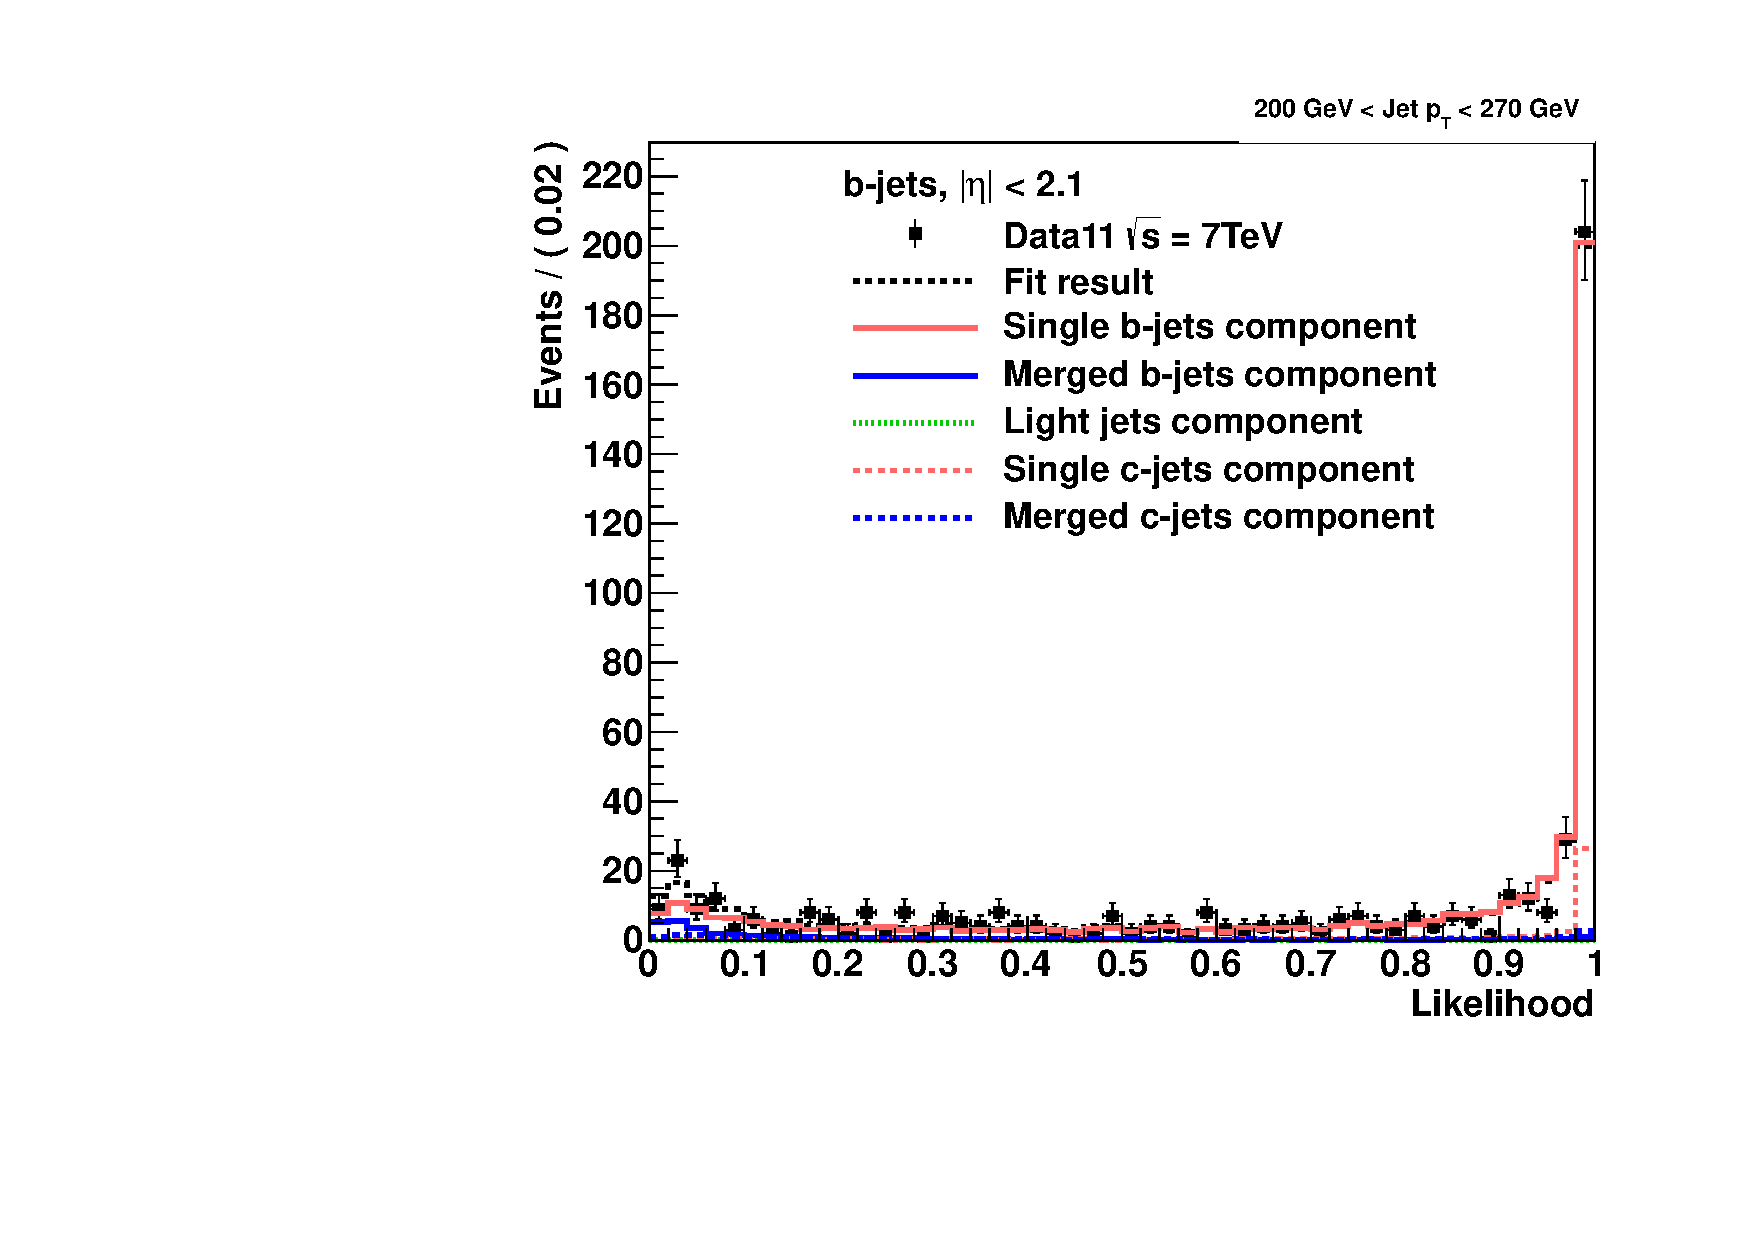
\includegraphics[width=0.7\textwidth]{FIGS/Fits/LikelihoodFit_3param_ETAFull_DataEnriched2btag_Bin5.pdf}
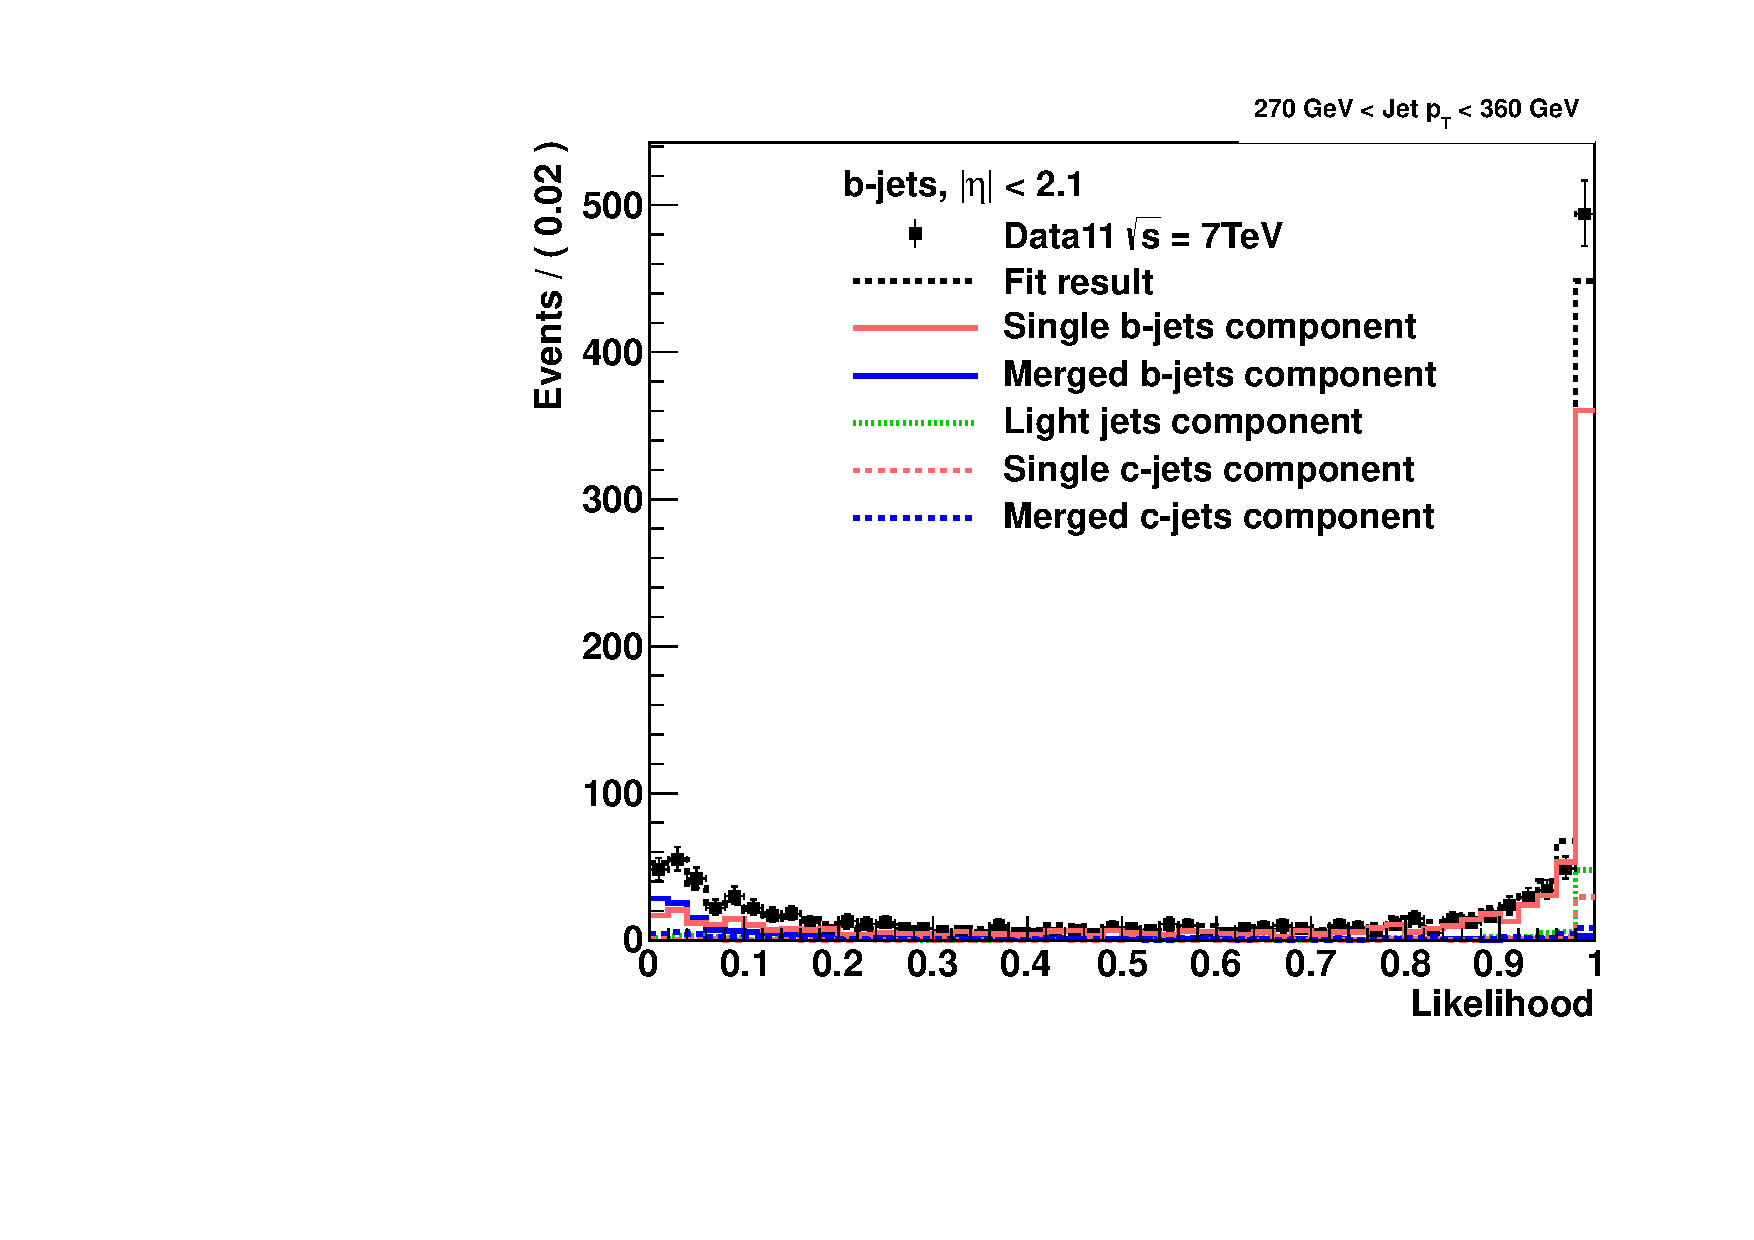
\includegraphics[width=0.7\textwidth]{FIGS/Fits/LikelihoodFit_3param_ETAFull_DataEnriched2btag_Bin6.pdf}
\caption{The results of template fits to the likelihood distribution in data enriched in single $b$-jets. The fits shown here were performed on jets with $\pt$ between  200~GeV and 270~GeV, and 270~GeV and 360~GeV, using five templates of $b$-, $b\bar{b}$-, $c$-, $c\bar{c}$, and light jets.  The ratio of the $c$- to $b$-flavour fractions was fixed to the values observed in the simulation.  Uncertainties shown are for data statistics only.}
\label{fig:fitenriched2btag2}
\end{figure}




\begin{table}[!hbt] %[h]
\renewcommand{\arraystretch}{1.2}
\centering
\begin{tabular}{ | c || c | c | c ||}
  \hline
  Jet $\pt$ & \multicolumn{3}{c||}{single $b$-jet}\\ \cline{2-4}
    (GeV ) & ~~~~fit result~~~ & ~~~~stat.err.~~~~ & pythia prediction \\ \hline
   40 - 60 &  99\%  &  11\%  &  84\% \\  
   60 - 80 &  82\%  &  ~5\%  &  87\% \\ 
   80 - 110&  84\%  &  ~5\%  &  88\% \\ 
  110 - 150&  86\%  &  ~8\%  &  85\% \\ 
  150 - 200&  89\%  &  ~9\%  &  83\% \\ 
  200 - 270&  95\%  &  15\%  &  80\% \\ 
  270 - 360&  67\%  &  11\%  &  81\% \\ 
  360 - 480&  73\%  &  16\%  &  73\% \\ \hline
\end{tabular}
\caption{Measured fractions of single $b$-jets in experimental data from 2011 run, enriched in single $b$-jets.}
\label{tb:fitfractions2btagS}
\end{table}

\begin{table}[!hbt] %[h]
\renewcommand{\arraystretch}{1.2}
\centering
\begin{tabular}{ | c || c | c | c ||}
  \hline
  Jet $\pt$ & \multicolumn{3}{c||}{merged $b$-jet}\\ \cline{2-4}
    (GeV ) & ~~~~fit result~~~ & ~~~~stat.err.~~~~ & pythia prediction \\ \hline
   40 - 60 &  -1\%  &  1\%  &  1\% \\  
   60 - 80 &  -3\%  &  1\%  &  1\% \\ 
   80 - 110&  ~2\%  &  1\%  &  1\% \\ 
  110 - 150&  ~4\%  &  2\%  &  3\% \\ 
  150 - 200&  ~4\%  &  2\%  &  3\% \\ 
  200 - 270&  ~7\%  &  2\%  &  5\% \\ 
  270 - 360&  12\%  &  2\%  &  6\% \\ 
  360 - 480&  10\%  &  1\%  &  8\% \\ \hline
\end{tabular}
\caption{Measured fractions of merged $b$-jets in experimental data from 2011 run, enriched in single $b$-jets.}
\label{tb:fitfractions2btagM}
\end{table}

\begin{table}[!hbt] %[h]
\renewcommand{\arraystretch}{1.2}
\centering
\begin{tabular}{ | c || c | c | c ||}
  \hline
  Jet $\pt$ & \multicolumn{3}{c||}{light $b$-jet}\\ \cline{2-4}
    (GeV ) & ~~~~fit result~~~ & ~~~~stat.err.~~~~ & pythia prediction \\ \hline
   40 - 60 &  ~-7\%  &  11\%  &  5\% \\  
   60 - 80 &  ~17\%  &  ~6\%  &  2\% \\ 
   80 - 110&  ~~4\%  &  ~6\%  &  1\% \\ 
  110 - 150&  ~-1\%  &  ~9\%  &  1\% \\ 
  150 - 200&  ~-6\%  &  10\%  &  2\% \\ 
  200 - 270&  -17\%  &  17\%  &  3\% \\ 
  270 - 360&  ~~9\%  &  11\%  &  4\% \\ 
  360 - 480&  ~~4\%  &  16\%  &  8\% \\ \hline
\end{tabular}
\caption{Measured fractions of light $b$-jets in experimental data from 2011 run, enriched in single $b$-jets.}
\label{tb:fitfractions2btagL}
\end{table}
